\protect\hyperlink{main-nav}{≡} \protect\hyperlink{close-nav}{×}

\hypertarget{section-3.7-applications-to-business}{%
\section{Section 3.7: Applications to
Business}\label{section-3.7-applications-to-business}}

\hypertarget{consumer-and-producer-surplus}{%
\subsection{Consumer and Producer
Surplus}\label{consumer-and-producer-surplus}}

Here are a demand and a supply curve for a product. Which is which?

\begin{figure}
\centering
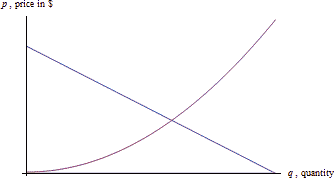
\includegraphics{images/image062.png}
\caption{}
\end{figure}

The demand curve is decreasing -- lower prices are associated with
higher quantities demanded, higher prices are associated with lower
quantities demanded. Demand curves are often shown as if they were
linear, but there's no reason they have to be.

The supply curve is increasing -- lower prices are associated with lower
supply, and higher prices are associated with higher quantities
supplied.

The point where the demand and supply curve cross is called the
equilibrium point \textbackslash{}((q\^{}*, p\^{}*)\textbackslash{}).

\begin{figure}
\centering
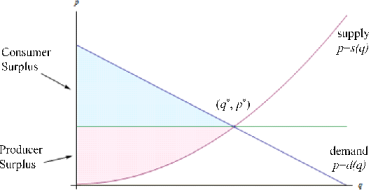
\includegraphics{images/image063.png}
\caption{}
\end{figure}

Suppose that the price is set at the equilibrium price, so that the
quantity demanded equals the quantity supplied. Now think about the
folks who are represented on the left of the equilibrium point. The
consumers on the left would have been willing to pay a higher price than
they ended up having to pay, so the equilibrium price saved them money.
On the other hand, the producers represented on the left would have been
willing to supply these goods for a lower price -- they made more money
than they expected to. Both of these groups ended up with extra cash in
their pockets!

Graphically, the amount of extra money that ended up in consumers'
pockets is the area between the demand curve and the horizontal line at
\textbackslash{}(p\^{}*\textbackslash{}). This is the difference in
price, summed up over all the consumers who spent less than they
expected to -- a definite integral. Notice that since the area under the
horizontal line is a rectangle, we can simplify the area integral:
\textbackslash{}{[}
\textbackslash{}int\textbackslash{}limits\_0\^{}\{q\^{}*\}
\textbackslash{}left( d(q)-p\^{}*\textbackslash{}right)\textbackslash{},
dq = \textbackslash{}int\textbackslash{}limits\_0\^{}\{q\^{}*\}
d(q)\textbackslash{}, dq -
\textbackslash{}int\textbackslash{}limits\_0\^{}\{q\^{}*\}
p\^{}*\textbackslash{}, dq =
\textbackslash{}int\textbackslash{}limits\_0\^{}\{q\^{}*\}
d(q)\textbackslash{}, dq - p\^{}*q\^{}*.\textbackslash{}{]}

The amount of extra money that ended up in producers' pockets is the
area between the supply curve and the horizontal line at
\textbackslash{}(p\^{}*\textbackslash{}). This is the difference in
price, summed up over all the producers who received more than they
expected to. Similar to consumer surplus, this integral can be
simplified: \textbackslash{}{[}
\textbackslash{}int\textbackslash{}limits\_0\^{}\{q\^{}*\}
\textbackslash{}left( p\^{}*-s(q)
\textbackslash{}right)\textbackslash{}, dq =
\textbackslash{}int\textbackslash{}limits\_0\^{}\{q\^{}*\}
p\^{}*\textbackslash{}, dq -
\textbackslash{}int\textbackslash{}limits\_0\^{}\{q\^{}*\}
s(q)\textbackslash{}, dq = p\^{}*q\^{}* -
\textbackslash{}int\textbackslash{}limits\_0\^{}\{q\^{}*\}
s(q)\textbackslash{}, dq.\textbackslash{}{]}

\hypertarget{consumer-and-producer-surplus-1}{%
\paragraph{Consumer and Producer
Surplus}\label{consumer-and-producer-surplus-1}}

Given a demand function \textbackslash{}(p = d(q)\textbackslash{}) and a
supply function \textbackslash{}(p = s(q)\textbackslash{}), and the
equilibrium point \textbackslash{}((q\^{}*, p\^{}*)\textbackslash{})

\begin{itemize}
\tightlist
\item
  The \textbf{consumer surplus} is
  \textbackslash{}{[}\textbackslash{}int\textbackslash{}limits\_0\^{}\{q\^{}*\}
  d(q)\textbackslash{}, dq - p\^{}*q\^{}*.\textbackslash{}{]}
\item
  The \textbf{producer surplus} is \textbackslash{}{[}p\^{}*q\^{}* -
  \textbackslash{}int\textbackslash{}limits\_0\^{}\{q\^{}*\}
  s(q)\textbackslash{}, dq.\textbackslash{}{]}
\item
  The sum of the consumer surplus and producer surplus is the
  \textbf{total gains from trade}.
\end{itemize}

What are the units of consumer and producer surplus? The units are
(price per item)(quantity of items) = money!

To view this video please enable JavaScript, and consider upgrading to a
web browser that \href{http://videojs.com/html5-video-support/}{supports
HTML5 video}

\hypertarget{example-1}{%
\paragraph{Example 1}\label{example-1}}

Suppose the demand for a product is given by \textbackslash{}(
p=d(q)=-0.8q+150 \textbackslash{}) and the supply for the same product
is given by \textbackslash{}( p=s(q)=5.2q \textbackslash{}). For both
functions, \textbackslash{}(q\textbackslash{}) is the quantity and
\textbackslash{}(p\textbackslash{}) is the price, in dollars.

\begin{enumerate}
\tightlist
\item
  Find the equilibrium point.
\item
  Find the consumer surplus at the equilibrium price.
\item
  Find the producer surplus at the equilibrium price.
\end{enumerate}

\begin{enumerate}
\tightlist
\item
  The equilibrium point is where the supply and demand functions are
  equal. Solving \textbackslash{}(-0.8q+150 = 5.2q\textbackslash{})
  gives \textbackslash{}(q = 25\textbackslash{}).
\item
  The consumer surplus is \textbackslash{}{[}
  \textbackslash{}int\textbackslash{}limits\_0\^{}\{25\}
  (-0.8q+150)\textbackslash{}, dq - (130)(25) = \textbackslash{}\$ 250.
  \textbackslash{}{]}
\item
  The producer surplus is \textbackslash{}{[} (130)(25) -
  \textbackslash{}int\textbackslash{}limits\_0\^{}\{25\}
  5.2q\textbackslash{}, dq = \textbackslash{}\$ 1625.
  \textbackslash{}{]}
\end{enumerate}

\hypertarget{example-2}{%
\paragraph{Example 2}\label{example-2}}

The tables below show information about the demand and supply functions
for a product. For both functions, \textbackslash{}(q\textbackslash{})
is the quantity and \textbackslash{}(p\textbackslash{}) is the price, in
dollars.

\begin{longtable}[]{@{}lllllllll@{}}
\toprule
\endhead
q & 0 & 100 & 200 & 300 & 400 & 500 & 600 & 700\tabularnewline
p & 70 & 61 & 53 & 46 & 40 & 35 & 31 & 28\tabularnewline
\bottomrule
\end{longtable}

\begin{longtable}[]{@{}lllllllll@{}}
\toprule
\endhead
q & 0 & 100 & 200 & 300 & 400 & 500 & 600 & 700\tabularnewline
p & 14 & 21 & 28 & 33 & 40 & 47 & 54 & 61\tabularnewline
\bottomrule
\end{longtable}

\begin{enumerate}
\tightlist
\item
  Which is which? That is, which table represents demand and which
  represents supply?
\item
  What is the equilibrium price and quantity?
\item
  Find the consumer and producer surplus at the equilibrium price.
\end{enumerate}

\begin{enumerate}
\item
  The first table shows decreasing price associated with increasing
  quantity; that is the demand function.
\item
  For both functions, \textbackslash{}(q = 400\textbackslash{}) is
  associated with \textbackslash{}(p = 40\textbackslash{}); the
  equilibrium price is \$40 and the equilibrium quantity is 400 units.
  Notice that we were lucky here, because the equilibrium point is
  actually one of the points shown. In many cases with a table, we would
  have to estimate.
\item
  The consumer surplus uses the demand function, which comes from the
  first table. We'll have to approximate the value of the integral using
  rectangles. There are 4 rectangles, and let's choose to use left
  endpoints.

  The consumer surplus is \textbackslash{}{[}
  \textbackslash{}begin\{align*\}
  \textbackslash{}int\textbackslash{}limits\_0\^{}\{400\}
  \textbackslash{}text\{(demand)\}\textbackslash{},
  dq-(40)(400)\textbackslash{}approx \& \textbackslash{}\textbackslash{}
  (100)(70+61+53+46)-(40)(400)=\& \textbackslash{}\$7000
  \textbackslash{}end\{align*\} \textbackslash{}{]} So the consumer
  surplus is about \$7000.

  The producer surplus uses the supply function, which comes from the
  second table. Let's choose to use left endpoints for this integral
  also.

  The producer surplus is \textbackslash{}{[}
  \textbackslash{}begin\{align*\}
  (40)(400)-\textbackslash{}int\textbackslash{}limits\_0\^{}\{400\}
  \textbackslash{}text\{(supply)\}\textbackslash{}, dq
  \textbackslash{}approx \& \textbackslash{}\textbackslash{}
  (40)(400)-(100)(14+21+28+33)=\& \textbackslash{}\$6400
  \textbackslash{}end\{align*\} \textbackslash{}{]} So the producer
  surplus is about \$6400.
\end{enumerate}

\hypertarget{continuous-income-stream}{%
\subsection{Continuous Income Stream}\label{continuous-income-stream}}

In precalculus, you learned about compound interest in that really
simple situation where you made a single deposit into an
interest-bearing account and let it sit undisturbed, earning interest,
for some period of time. Recall:

\hypertarget{compound-interest-formulas}{%
\paragraph{Compound Interest
Formulas}\label{compound-interest-formulas}}

Let \textbackslash{}(P\textbackslash{}) be the principal (initial
investment), \textbackslash{}(r\textbackslash{}) be the annual interest
rate expressed as a decimal, and \textbackslash{}(A(t)\textbackslash{})
be the amount in the account at the end of
\textbackslash{}(t\textbackslash{}) years.

\hypertarget{compounding-n-times-per-year}{%
\subparagraph{Compounding \textbackslash{}(n\textbackslash{}) times per
year}\label{compounding-n-times-per-year}}

\textbackslash{}{[} A(t) =
P\textbackslash{}left(1+\textbackslash{}frac\{r\}\{n\}\textbackslash{}right)\^{}\{nt\}
\textbackslash{}{]}

\hypertarget{compounded-continuously}{%
\subparagraph{Compounded continuously}\label{compounded-continuously}}

\textbackslash{}{[} A(t)=Pe\^{}\{rt\} \textbackslash{}{]}

If you're using this formula to find what an account will be worth in
the future, \textbackslash{}(t \textbackslash{}gt 0\textbackslash{}) and
\textbackslash{}(A(t)\textbackslash{}) is called the \textbf{future
value}.

If you're using the formula to find what you need to deposit today to
have a certain value \textbackslash{}(P\textbackslash{}) sometime in the
future, \textbackslash{}(t \textbackslash{}lt 0\textbackslash{}) and
\textbackslash{}(A(t)\textbackslash{}) is called the \textbf{present
value}.

You may also have learned somewhat more complicated annuity formulas to
deal with slightly more complicated situations -- where you make equal
deposits equally spaced in time.

But real life is not usually so neat.

Calculus allows us to handle situations where ``deposits'' are flowing
continuously into an account that earns interest. As long as we can
model the flow of income with a function, we can use a definite integral
to calculate the present and future value of a continuous income stream.
The idea here is that each little bit of income in the future needs to
be multiplied by the exponential function to bring it back to the
present, and then we'll add them all up (a definite integral).

\hypertarget{continuous-income-stream-1}{%
\paragraph{Continuous Income Stream}\label{continuous-income-stream-1}}

Suppose money can earn interest at an annual interest rate of r,
compounded continuously. Let F(t) be a continuous income function (in
dollars per year) that applies between year 0 and year T.

Then the present value of that income stream is given by
\textbackslash{}{[} PV =
\textbackslash{}int\textbackslash{}limits\_0\^{}T
F(t)e\^{}\{-rt\}\textbackslash{}, dt. \textbackslash{}{]}

The future value can be computed by the ordinary compound interest
formula \textbackslash{}{[} FV = PVe\^{}\{rt\}. \textbackslash{}{]}

This is a useful way to compare two investments -- find the present
value of each to see which is worth more today.

To view this video please enable JavaScript, and consider upgrading to a
web browser that \href{http://videojs.com/html5-video-support/}{supports
HTML5 video}

\hypertarget{example-3}{%
\paragraph{Example 3}\label{example-3}}

You have an opportunity to buy a business that will earn \$75,000 per
year continuously over the next eight years. Money can earn 2.8\% per
year, compounded continuously. Is this business worth its purchase price
of \$630,000?

First, please note that we still have to make some simplifying
assumptions. We have to assume that the interest rates are going to
remain constant for that entire eight years. We also have to assume that
the \$75,000 per year is coming in continuously, like a faucet dripping
dollars into the business. Neither of these assumptions might be
accurate.

But moving on: The present value of the \$630,000 is, well, \$630,000.
This is one investment, where we put our \$630,000 in the bank and let
it sit there.

To find the present value of the business, we think of it as an income
stream. The function \textbackslash{}(F(t)\textbackslash{}) in this case
is a constant \$75,000 dollars per year, so \textbackslash{}(F(t) =
75,\textbackslash{}!000\textbackslash{}). The interest rate is 2.8\% and
the term we're interested in is 8 years, so \textbackslash{}(r =
.028\textbackslash{}), and \textbackslash{}(T = 8\textbackslash{}):
\textbackslash{}{[} PV=\textbackslash{}int\textbackslash{}limits\_0\^{}8
75000e\^{}\{-0.028t\}\textbackslash{}, dt \textbackslash{}approx
537,\textbackslash{}!548.75 \textbackslash{}{]}

The present value of the business is about \$537,500, which is less than
the \$630,000 asking price, so this is not a good deal.

While this integral could have been done using substitution, for many of
the integrals in this section we don't have the techniques to use
antiderivatives or, in some cases, no antiderivative exists. Technology
will work quickly, and it will give you an answer that is good enough.

\hypertarget{example-4}{%
\paragraph{Example 4}\label{example-4}}

A company is considering purchasing a new machine for its production
floor. The machine costs \$65,000. The company estimates that the
additional income from the machine will be a constant \$7000 for the
first year, then will increase by \$800 each year after that. In order
to buy the machine, the company needs to be convinced that it will pay
for itself by the end of 8 years with this additional income. Money can
earn 1.7\% per year, compounded continuously. Should the company buy the
machine?

We'll assume that the income will come in continuously over the 8 years.
We'll also assume that interest rates will remain constant over that
8-year time period.

We're interested in the present value of the machine, which we will
compare to its \$65,000 price tag. Let
\textbackslash{}(t\textbackslash{}) be the time, in years, since the
purchase of the machine. The income from the machine is different
depending on the time.

From \textbackslash{}(t = 0\textbackslash{}) to \textbackslash{}(t =
1\textbackslash{}) (the first year), the income is constant \$7000 per
year. From \textbackslash{}(t = 1\textbackslash{}) to \textbackslash{}(t
= 8\textbackslash{}), the income is increasing by \$800 each year; the
income flow function \textbackslash{}(F(t)\textbackslash{}) will be
\textbackslash{}( F(t)=7000+800(t-1)=6200+800t \textbackslash{}). To
find the present value, we'll have to divide the integral into the two
pieces, one for each of the functions: \textbackslash{}{[}
PV=\textbackslash{}int\textbackslash{}limits\_0\^{}1
7000e\^{}\{-0.017t\}\textbackslash{}, dt +
\textbackslash{}int\textbackslash{}limits\_1\^{}8
(6200+800t)e\^{}\{-0.017t\}\textbackslash{}, dt \textbackslash{}approx
70166. \textbackslash{}{]}

The present value is greater than the cost of the machine, so the
company should buy the machine.

\begin{longtable}[]{@{}ll@{}}
\toprule
\endhead
\href{section3-6.php}{← Previous Section} & \href{section3-8.php}{Next
Section →}\tabularnewline
\bottomrule
\end{longtable}
